\documentclass[lettersize,journal]{IEEEtran}
\usepackage{amsmath,amsfonts}
\usepackage{algorithmic}
\usepackage{algorithm}
\usepackage{array}
\usepackage[caption=false,font=normalsize,labelfont=sf,textfont=sf]{subfig}
\usepackage{textcomp}
\usepackage{stfloats}
\usepackage{url}
\usepackage{verbatim}
\usepackage{graphicx}
\usepackage{cite}

\usepackage{microtype}
\usepackage{booktabs}
\usepackage{siunitx}
\usepackage{tabularx}
\usepackage{tikz}
\usetikzlibrary{positioning, arrows.meta, automata, fit, backgrounds, calc}
\newtheorem{definition}{Definition}
\newtheorem{proposition}{Proposition}

\hyphenation{op-tical net-works semi-conduc-tor IEEE-Xplore}
% updated with editorial comments 8/9/2021

\begin{document}

\title{CTAP2.1 on Zephyr RTOS: Design and Multi-Platform Evaluation of an Open-Source FIDO2 Authenticator}

\author{
    Md~Siratul~Islam
    and~Md~Rasedujjaman
    \thanks{Md Siratul Islam is with the Department of Physics, Shahjalal University of Science and Technology, Sylhet 3114, Bangladesh (e-mail: email@sirat.me).}
    \thanks{Md Rasedujjaman is with the Department of Electrical and Electronic Engineering, Shahjalal University of Science and Technology, Sylhet 3114, Bangladesh.}
}

% The paper headers
\markboth{IEEE Transactions on Information Forensics and Security,~Vol.~14, No.~8, August~2021}%
{S. Islam and M. Rasedujjaman: CTAP2.1 on Zephyr RTOS: Design and Multi-Platform Evaluation of an Open-Source FIDO2 Authenticator}

\IEEEpubid{0000--0000/00\$00.00~\copyright~2021 IEEE}
% Remember, if you use this you must call \IEEEpubidadjcol in the second
% column for its text to clear the IEEEpubid mark.

\maketitle

\begin{abstract}
This document describes the most common article elements and how to use the IEEEtran class with \LaTeX \ to produce files that are suitable for submission to the IEEE.  IEEEtran can produce conference, journal, and technical note (correspondence) papers with a suitable choice of class options.
\end{abstract}

\begin{IEEEkeywords}
Article submission, IEEE, IEEEtran, journal, \LaTeX, paper, template, typesetting.
\end{IEEEkeywords}

\input{sections/01_introduction}
\newpage

\input{sections/02_related}
\section{Formal Model}
\label{sec:formal}

\subsection{Automaton Definition}
\label{sec:formal:def}

We model the CTAP2.1 authenticator as a deterministic finite automaton~(DFA) $\mathcal{M} = (Q,\,\Sigma,\,\delta,\,q_0,\,F)$ whose states correspond directly to observable execution phases in the Zephyr implementation. Table~\ref{tab:dfa-summary} summarises the three principal components of $\mathcal{M}$.

\begin{table}[t]
\renewcommand{\arraystretch}{1.2}
\caption{CTAP2.1 Authenticator DFA Summary}
\label{tab:dfa-summary}
\centering
\begin{tabular}{@{}lll@{}}
\toprule
Component & Count & Categories \\
\midrule
$Q$ & 30 &
  Lifecycle (2), Dispatch (1), \\[-1pt]
  & & \texttt{MakeCredential} sub-states (13), \\[-1pt]
  & & \texttt{GetAssertion} sub-states (9), \\[-1pt]
  & & \texttt{GetNextAssertion} sub-states (2), \\[-1pt]
  & & Simple commands (2), \texttt{SEND} (1) \\[3pt]
$\Sigma$ & 26 &
  Lifecycle events (2), command bytes (7), \\[-1pt]
  & & operation outcomes (17) \\[3pt]
$F$ & 2 & \texttt{STOPPED},\ \texttt{IDLE} \\
\bottomrule
\end{tabular}
\end{table}

\begin{definition}[CTAP2.1 Authenticator Automaton]
\label{def:dfa}
The FIDO2/CTAP2.1 authenticator is modeled as $\mathcal{M} = (Q,\,\Sigma,\,\delta,\,q_0,\,F)$ where: $Q$ is the set of 30 execution states in Table~\ref{tab:dfa-summary}; $\Sigma$ is the 26-symbol alphabet comprising lifecycle events $\{\mathtt{start},\mathtt{stop}\}$, command bytes $\{\mathtt{cmd\_01},\mathtt{cmd\_02},\mathtt{cmd\_04}, \mathtt{cmd\_07},\mathtt{cmd\_08},\mathtt{cmd\_0B}, \mathtt{cmd\_xx}\}$, and operation outcomes $\{\mathtt{cbor\_ok},\mathtt{cbor\_fail},\mathtt{up\_ok}, \mathtt{up\_timeout},\mathtt{up\_cancel},\mathtt{ok}, \mathtt{fail},\mathtt{excluded},\mathtt{not\_excl}, \mathtt{rk},\mathtt{not\_rk},\mathtt{found}, \mathtt{not\_found},\mathtt{pending},\mathtt{not\_pending}, \mathtt{multi},\mathtt{msg}\}$; $\delta : Q \times \Sigma \rightarrow Q$ is the total transition function with representative entries in Table~\ref{tab:impl-map}; $q_0 = \mathtt{STOPPED}$ is the initial state set at static initialisation; and $F = \{\mathtt{STOPPED},\,\mathtt{IDLE}\}$ is the set of accepting states.
\end{definition}

\subsection{Composite Structure}
\label{sec:formal:composite}

The MakeCredential, GetAssertion, and GetNextAssertion
sub-automata share a common terminal state \texttt{SEND},
which unconditionally executes
\texttt{transport\allowbreak->api\allowbreak->send()},
issues \texttt{notify(FIDO2\_WIRE\_STATUS\_DONE)}, and
transitions to \texttt{IDLE}.
Fig.~\ref{fig:composite-dfa} shows the full flattened
composite automaton.
The dispatch state \texttt{DISPATCH} routes on the command
byte to the entry state of the appropriate sub-machine;
unknown bytes route directly to \texttt{SEND} with status
\texttt{FIDO2\_ERR\_INVALID\_COMMAND}.
This structure guarantees that every execution path
terminates at \texttt{IDLE} through a single well-defined
send transition.

\begin{figure*}[t]
\centering
\resizebox{\linewidth}{!}{%
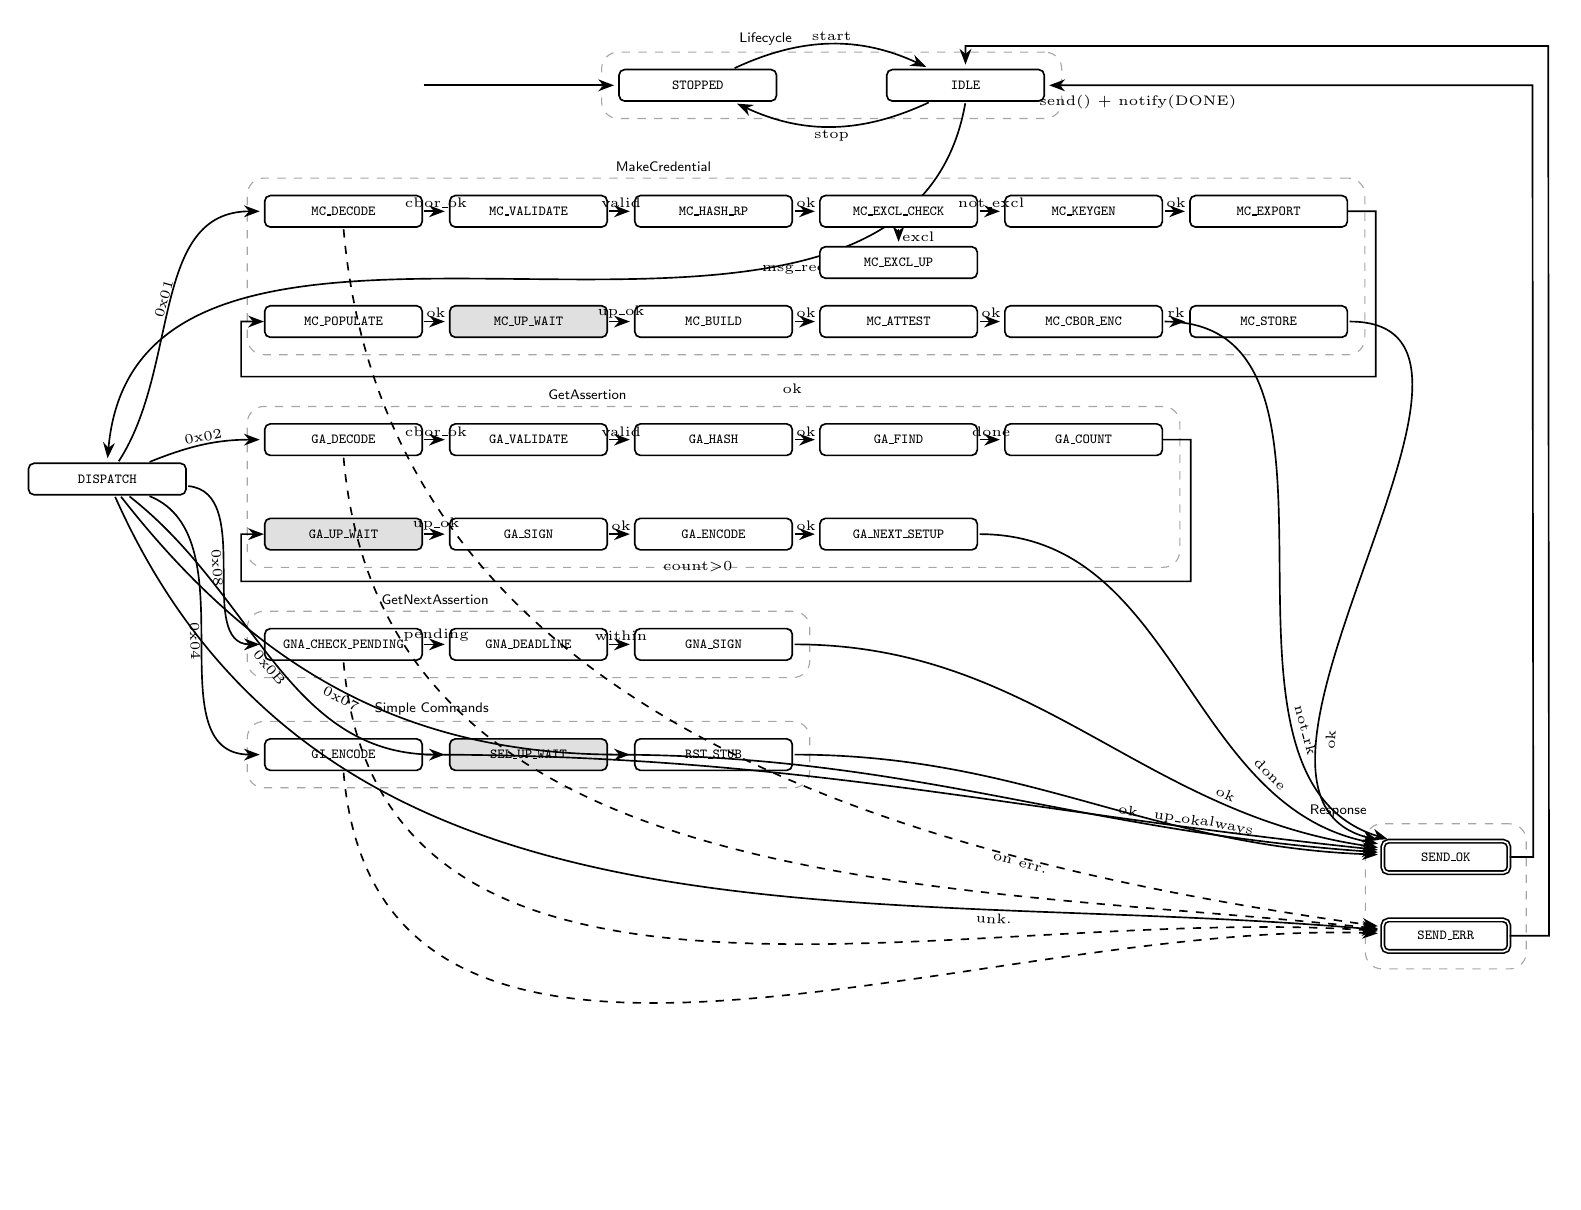
\begin{tikzpicture}[
  ->, >=Stealth, shorten >=1.5pt, shorten <=0.5pt, semithick,
  % Normal state
  st/.style   = {draw, rounded corners=2pt,
                 minimum width=2.0cm, minimum height=0.40cm,
                 font=\tiny\ttfamily, fill=white, inner sep=2pt},
  % UP-wait state — shaded to reference Proposition 3
  upst/.style = {draw, rounded corners=2pt,
                 minimum width=2.0cm, minimum height=0.40cm,
                 font=\tiny\ttfamily, fill=black!12, inner sep=2pt},
  % Accept state (double border)
  acc/.style  = {draw, double, distance=1.2pt, rounded corners=2pt,
                 minimum width=1.6cm, minimum height=0.40cm,
                 font=\tiny\ttfamily, fill=white, inner sep=2pt},
  % Group bounding box
  grp/.style  = {draw=black!35, dashed, rounded corners=6pt,
                 inner sep=6pt},
  % Edge label
  lbl/.style  = {font=\tiny, inner sep=1pt},
]

%%----------------------------------------------------------------
%% COORDINATE MAP
%%   Horizontal step (state centres): 2.35 cm
%%   x1=3.00  x2=5.35  x3=7.70  x4=10.05  x5=12.40  x6=14.75
%%   xS=17.0  (SEND_OK / SEND_ERR)
%%
%%   y_lc   = 15.5   Lifecycle
%%   y_disp = 13.8   DISPATCH
%%   y_mc1  = 12.4   MC row 1
%%   y_mcb  = 11.75  MC_EXCL_UP branch
%%   y_mc2  = 11.0   MC row 2
%%   y_ga1  =  9.5   GA row 1
%%   y_ga2  =  8.3   GA row 2
%%   y_gna  =  6.9   GetNextAssertion
%%   y_sim  =  5.5   Simple commands
%%   y_sok  =  4.2   SEND_OK
%%   y_ser  =  3.2   SEND_ERR
%%----------------------------------------------------------------

%% =================== LIFECYCLE ================================
\node[st] (STOP) at ( 7.5, 14) {STOPPED};
\node[st] (IDLE) at ( 10.9, 14) {IDLE};
\draw[->] (4, 14) -- (STOP.west);
\draw (STOP) to[bend left=25] node[lbl, above]{start} (IDLE);
\draw (IDLE) to[bend left=25] node[lbl, below]{stop}  (STOP);

%% =================== DISPATCH =================================
\node[st] (DISP) at (0, 9) {DISPATCH};
\draw (IDLE.south) to[out=-100, in=85]
    node[lbl, right, pos=0.3]{msg\_recv} (DISP.north);

%% =================== MC ROW 1  (y=12.4) ======================
\node[st]   (MCDEC) at ( 3.00, 12.4) {MC\_DECODE};
\node[st]   (MCVAL) at ( 5.35, 12.4) {MC\_VALIDATE};
\node[st]   (MCHRP) at ( 7.70, 12.4) {MC\_HASH\_RP};
\node[st]   (MCEXC) at (10.05, 12.4) {MC\_EXCL\_CHECK};
\node[st]   (MCKG)  at (12.40, 12.4) {MC\_KEYGEN};
\node[st]   (MCEXP) at (14.75, 12.4) {MC\_EXPORT};
% branch state
\node[st]   (MCEUP) at (10.05, 11.75) {MC\_EXCL\_UP};

%% Row 1 transitions
\draw (MCDEC) -- node[lbl, above]{cbor\_ok}   (MCVAL);
\draw (MCVAL) -- node[lbl, above]{valid}      (MCHRP);
\draw (MCHRP) -- node[lbl, above]{ok}         (MCEXC);
\draw (MCEXC) -- node[lbl, above]{not\_excl}  (MCKG);
\draw (MCEXC) -- node[lbl, right]{excl}       (MCEUP);
\draw (MCKG)  -- node[lbl, above]{ok}         (MCEXP);

%% =================== MC ROW 2  (y=11.0) ======================
\node[st]   (MCPOP) at ( 3.00, 11.0) {MC\_POPULATE};
\node[upst] (MCUPW) at ( 5.35, 11.0) {MC\_UP\_WAIT};
\node[st]   (MCBLD) at ( 7.70, 11.0) {MC\_BUILD};
\node[st]   (MCATT) at (10.05, 11.0) {MC\_ATTEST};
\node[st]   (MCENC) at (12.40, 11.0) {MC\_CBOR\_ENC};
\node[st]   (MCSTR) at (14.75, 11.0) {MC\_STORE};

%% Fold: MC_EXPORT (row1 end) → MC_POPULATE (row2 start)
%% Path: right from MCEXP → down to y=10.3 (below row2) → left → up into MCPOP
\draw[shorten >=0pt, shorten <=0pt]
    (MCEXP.east)
    -- ++(0.35, 0)
    -- ++(0,   -2.1)         %% down to y=10.3
    -- (1.7, 10.3)          %% left to just before MCPOP
    -- (1.7, 11.0)          %% up to row2 y
    -- (MCPOP.west);
\node[lbl, below] at (8.7, 10.25) {ok};   %% label on horizontal segment

%% Row 2 transitions
\draw (MCPOP) -- node[lbl, above]{ok}     (MCUPW);
\draw (MCUPW) -- node[lbl, above]{up\_ok} (MCBLD);
\draw (MCBLD) -- node[lbl, above]{ok}     (MCATT);
\draw (MCATT) -- node[lbl, above]{ok}     (MCENC);
\draw (MCENC) -- node[lbl, above]{rk}     (MCSTR);

%% =================== GA ROW 1  (y=9.5) =======================
\node[st]   (GADEC) at ( 3.00, 9.5) {GA\_DECODE};
\node[st]   (GAVAL) at ( 5.35, 9.5) {GA\_VALIDATE};
\node[st]   (GAHSH) at ( 7.70, 9.5) {GA\_HASH};
\node[st]   (GAFND) at (10.05, 9.5) {GA\_FIND};
\node[st]   (GACNT) at (12.40, 9.5) {GA\_COUNT};

%% Row 1 transitions
\draw (GADEC) -- node[lbl, above]{cbor\_ok} (GAVAL);
\draw (GAVAL) -- node[lbl, above]{valid}    (GAHSH);
\draw (GAHSH) -- node[lbl, above]{ok}       (GAFND);
\draw (GAFND) -- node[lbl, above]{done}     (GACNT);

%% =================== GA ROW 2  (y=8.3) =======================
\node[upst] (GAUPW) at ( 3.00, 8.3) {GA\_UP\_WAIT};
\node[st]   (GASNG) at ( 5.35, 8.3) {GA\_SIGN};
\node[st]   (GAENC) at ( 7.70, 8.3) {GA\_ENCODE};
\node[st]   (GANXT) at (10.05, 8.3) {GA\_NEXT\_SETUP};

%% Fold: GA_COUNT → GA_UP_WAIT
\draw[shorten >=0pt, shorten <=0pt]
    (GACNT.east)
    -- ++(0.35, 0)
    -- ++(0,   -1.8)        %% down to y=8.05
    -- (1.7,   7.7)
    -- (1.7,   8.3)
    -- (GAUPW.west);
\node[lbl, below] at (7.5, 8.0) {count>0};

%% Row 2 transitions
\draw (GAUPW) -- node[lbl, above]{up\_ok} (GASNG);
\draw (GASNG) -- node[lbl, above]{ok}     (GAENC);
\draw (GAENC) -- node[lbl, above]{ok}     (GANXT);

%% =================== GetNextAssertion  (y=6.9) ================
\node[st] (GNACHK) at ( 3.00, 6.9) {GNA\_CHECK\_PENDING};
\node[st] (GNADL)  at ( 5.35, 6.9) {GNA\_DEADLINE};
\node[st] (GNASNG) at ( 7.70, 6.9) {GNA\_SIGN};

\draw (GNACHK) -- node[lbl, above]{pending} (GNADL);
\draw (GNADL)  -- node[lbl, above]{within}  (GNASNG);

%% =================== Simple Commands  (y=5.5) =================
\node[st]   (GIENC)  at (3.00, 5.5) {GI\_ENCODE};
\node[upst] (SELUP)  at (5.35, 5.5) {SEL\_UP\_WAIT};
\node[st]   (RSTSTB) at (7.70, 5.5) {RST\_STUB};

%% =================== TERMINAL STATES =========================
\node[acc] (SNOK) at (17.0, 4.2) {SEND\_OK};
\node[acc] (SNER) at (17.0, 3.2) {SEND\_ERR};

%% =================== RESPONSE → IDLE FEEDBACK ================
%% Route: right edge → up to y=16.8 (above LC) → left to IDLE.north
\draw[shorten >=1.5pt, shorten <=0pt]
    (SNOK.east)
    -- ++(0.3, 0)
    -- (18.1, 14)
    -- (12.5,  14)
    -- (IDLE.east)
    node[pos=-1, below, font=\tiny]{send() + notify(DONE)};

\draw[shorten >=1.5pt, shorten <=0pt]
    (SNER.east)
    -- ++(0.5, 0)
    -- (18.3, 14.5)
    -- (10.9,  14.5)
    -- (IDLE.north);        %% shares label with SNOK path; no extra label

%% =================== DISPATCH FANOUT =========================
\draw (DISP) to[out=57,  in=180]
    node[lbl, above, sloped, pos=0.5]{0x01} (MCDEC);
\draw (DISP) to[out=22,  in=180]
    node[lbl, above, sloped, pos=0.5]{0x02} (GADEC);
\draw (DISP) to[out=-5,  in=180]
    node[lbl, below, sloped, pos=0.5]{0x08} (GNACHK);
\draw (DISP) to[out=-22, in=180]
    node[lbl, below, sloped, pos=0.5]{0x04} (GIENC);
\draw (DISP) to[out=-38, in=180]
    node[lbl, below, sloped, pos=0.5]{0x0B} (SELUP);
\draw (DISP) to[out=-52, in=180]
    node[lbl, below, sloped, pos=0.5]{0x07} (RSTSTB);
\draw (DISP) to[out=-66, in=175]
    node[lbl, below, sloped, near end]{unk.} (SNER);

%% =================== SUCCESS → SEND_OK =======================
\draw (MCENC) to[out=0, in=163]
    node[lbl, above, sloped, near end]{not\_rk} (SNOK);
\draw (MCSTR) to[out=0, in=166]
    node[lbl, below, sloped, near end]{ok}      (SNOK);
\draw (GANXT) to[out=0, in=169]
    node[lbl, above, sloped, near end]{done}    (SNOK);
\draw (GNASNG) to[out=0, in=172]
    node[lbl, above, sloped, near end]{ok}      (SNOK);
\draw (GIENC)  to[out=0, in=174]
    node[lbl, above, sloped, near end]{ok}      (SNOK);
\draw (SELUP)  to[out=0, in=176]
    node[lbl, above, sloped, near end]{up\_ok}  (SNOK);
\draw (RSTSTB) to[out=0, in=178]
    node[lbl, above, sloped, near end]{always}  (SNOK);

%% =================== ERROR → SEND_ERR ========================
%% One dashed arrow per sub-machine (individual error labels
%% omitted; full list in Table~\ref{tab:impl-map})
\draw[dashed, ->] (MCDEC.south)
    to[out=-85, in=172]
    node[lbl, below, sloped, near end]{on err.} (SNER);
\draw[dashed, ->] (GADEC.south)
    to[out=-85, in=174]
    (SNER);
\draw[dashed, ->] (GNACHK.south)
    to[out=-85, in=176]
    (SNER);
\draw[dashed, ->] (GIENC.south)
    to[out=-85, in=178]
    (SNER);

%% =================== GROUP BOXES =============================
\begin{scope}[on background layer]

\node[grp,
    fit=(STOP)(IDLE),
    label={[font=\tiny\sffamily, inner sep=2pt]above left:Lifecycle}]
    {};

\node[grp,
    fit=(MCDEC)(MCVAL)(MCHRP)(MCEXC)(MCEUP)(MCKG)(MCEXP)%
        (MCPOP)(MCUPW)(MCBLD)(MCATT)(MCENC)(MCSTR),
    label={[font=\tiny\sffamily, inner sep=2pt]above left:MakeCredential}]
    (MCBOX) {};

\node[grp,
    fit=(GADEC)(GAVAL)(GAHSH)(GAFND)(GACNT)(GAUPW)(GASNG)(GAENC)(GANXT),
    label={[font=\tiny\sffamily, inner sep=2pt]above left:GetAssertion}]
    (GABOX) {};

\node[grp,
    fit=(GNACHK)(GNADL)(GNASNG),
    label={[font=\tiny\sffamily, inner sep=2pt]above left:GetNextAssertion}]
    {};

\node[grp,
    fit=(GIENC)(SELUP)(RSTSTB),
    label={[font=\tiny\sffamily, inner sep=2pt]above left:Simple Commands}]
    {};

\node[grp,
    fit=(SNOK)(SNER),
    label={[font=\tiny\sffamily, inner sep=2pt]above left:Response}]
    {};

\end{scope}

\end{tikzpicture}%
}
\caption{Composite CTAP2.1 DFA~$\mathcal{M}$ with qualified
         per-command sub-states.
         Shaded nodes (\texttt{MC\_UP\_WAIT},
         \texttt{GA\_UP\_WAIT}, \texttt{SEL\_UP\_WAIT}) are
         the gate states of Proposition~\ref{prop:up}:
         no successful credential path bypasses them.
         Dashed edges denote collective error transitions
         from each sub-machine to \texttt{SEND\_ERR};
         individual error labels are omitted for clarity.
         Fold arrows route below each band.
         Both terminal states return to \texttt{IDLE}
         via the right-side feedback path
         (\texttt{transport->api->send()} + \texttt{notify(DONE)}).
         Full state-to-source-line mapping in
         Table~\ref{tab:impl-map}.}
\label{fig:composite-dfa}
\end{figure*}

\subsection{Security and Correctness Properties}
\label{sec:formal:props}

\begin{proposition}[Determinism]
\label{prop:determinism}
For all $q \in Q$ and $\sigma \in \Sigma$,
$\delta(q,\,\sigma)$ is unique.
\end{proposition}
\IEEEproof
\texttt{process\_command()} is a \texttt{switch} statement
with non-overlapping \texttt{case} labels.
Each sub-handler follows a linear execution path with a
single error edge to \texttt{SEND} and a single success
edge to the next sub-state.
No state in Table~\ref{tab:impl-map} carries two outgoing
edges on the same input symbol.
\IEEEQED

\begin{proposition}[Completeness]
\label{prop:completeness}
$\delta$ is total: for all $q \in Q$ and
$\sigma \in \Sigma$, $\delta(q,\,\sigma)$ is defined.
\end{proposition}
\IEEEproof
Unknown command bytes are consumed by the \texttt{default}
branch of \texttt{process\_command()}, transitioning to
$\mathtt{SEND} \to \mathtt{IDLE}$ with status
\texttt{FIDO2\_ERR\_INVALID\_COMMAND}.
Every sub-state carries an explicit error edge to
\texttt{SEND} on any failure outcome.
No undefined $(q,\,\sigma)$ pair exists in
$Q \times \Sigma$.
\IEEEQED

\begin{proposition}[User Presence Isolation]
\label{prop:up}
Every execution path through a credential operation
that reaches \texttt{SEND} with status \texttt{FIDO2\_OK}
must pass through \texttt{MC\_UP\_WAIT} or
\texttt{GA\_UP\_WAIT}, respectively.
\end{proposition}
\IEEEproof
From Fig.~\ref{fig:composite-dfa}, the sole incoming edges
to \texttt{SEND} carrying \texttt{FIDO2\_OK} from
\texttt{MC}-prefixed states originate at \texttt{MC\_STORE}
and \texttt{MC\_CBOR\_ENC}.
Both are reachable only from \texttt{MC\_BUILD}, which
requires the $\mathtt{up\_ok}$ transition out of
\texttt{MC\_UP\_WAIT}.
No path from \texttt{MC\_DECODE} to a successful
\texttt{SEND} exists that bypasses \texttt{MC\_UP\_WAIT}.
The symmetric argument holds for \texttt{GA}-prefixed
states via \texttt{GA\_UP\_WAIT}.
\IEEEQED

\begin{proposition}[Sign Counter Monotonicity]
\label{prop:counter}
For credential $c$ with $\mathit{sign\_count}(c) = n$
prior to entering \texttt{GA\_SIGN}, upon completion
$\mathit{sign\_count}(c) \geq n + 1$ regardless of
power loss during \texttt{GA\_SIGN}.
\end{proposition}
\IEEEproof
\texttt{fido2\_storage\_sign\_count\_increment()} commits
the updated counter to NVS before returning.
Write-ahead ordering guarantees the counter is durable on
flash before the response is encoded.
A power loss during \texttt{GA\_SIGN} therefore leaves the
counter at $n+1$ upon recovery.
The storage API exposes no decrement path; the counter is
strictly non-decreasing across power cycles, satisfying the
WebAuthn Level~3~\cite{webauthn-l3} \S6.1.1
clone-detection requirement.
\IEEEQED

\begin{proposition}[Non-Discoverable Credential Opacity]
\label{prop:opacity}
A non-discoverable credential identifier observed on the
wire is computationally indistinguishable from a uniformly
random bitstring without access to the device-bound
AES-GCM wrapping key.
\end{proposition}
\IEEEproof
Non-discoverable credential identifiers are produced by
\texttt{fido2\_crypto\_wrap\_credential()}, which encrypts
the PSA key handle under a 256-bit device-bound AES-GCM key
in PSA persistent storage, with $\mathit{rp\_id\_hash}$ as
authenticated additional data~(AAD).
The AAD binding causes unwrap attempts under a mismatched
relying party context to yield an authentication tag failure
rather than a silently incorrect key handle.
Under the IND-CPA security of AES-GCM~\cite{iwata-gcm}
with a fresh per-operation nonce generated via
\texttt{psa\_generate\_random()}, an adversary without
physical device access cannot distinguish the 64-byte
ciphertext from a uniform random bitstring, and cannot
recover the wrapped key handle or the relying party binding.
\IEEEQED

\begin{proposition}[Deadlock and Livelock Freedom]
\label{prop:deadlock}
$\mathcal{M}$ contains no deadlock states and no livelock
cycles.
\end{proposition}
\IEEEproof
Deadlock freedom follows from
Proposition~\ref{prop:completeness}: every state in $Q$
has at least one defined outgoing transition.
For livelock, every cycle in the transition graph passes
through \texttt{IDLE}, which requires dequeuing a message
via \texttt{k\_msgq\_get(K\_MSEC(100))}.
Without an externally-sourced message the FIDO2 thread
blocks and yields the CPU; it cannot spin on an internal
transition.
No cycle bypassing \texttt{IDLE} exists, as confirmed by
inspection of Fig.~\ref{fig:composite-dfa}.
\IEEEQED

\begin{table}[t]
\renewcommand{\arraystretch}{1.2}
\caption{Representative DFA State to Source Code Mapping}
\label{tab:impl-map}
\centering
\small
\begin{tabular}{@{}lll@{}}
\toprule
State & \texttt{fido2\_core.c} & Role \\
\midrule
\texttt{STOPPED}      & L.\,69  & Static init, thread inactive \\
\texttt{IDLE}         & L.\,790 & Message queue poll \\
\texttt{DISPATCH}     & L.\,723 & \texttt{process\_command()} \\
\texttt{MC\_UP\_WAIT} & L.\,355 & \texttt{fido2\_up\_wait()} \\
\texttt{MC\_STORE}    & L.\,401 & NVS credential write \\
\texttt{GA\_FIND}     & L.\,414 & Length-based allowList dispatch \\
\texttt{GA\_SIGN}     & L.\,449 & Counter increment + ECDSA \\
\texttt{GNA\_CHECK}   & L.\,680 & Pending flag + 30\,s deadline \\
\texttt{SEND\_OK}     & L.\,809 & \texttt{send()} + \texttt{notify(DONE)} \\
\texttt{SEND\_ERR}    & L.\,809 & Error status + \texttt{notify(DONE)} \\
\bottomrule
\end{tabular}
\end{table}

\subsection{Security Implications}
\label{sec:formal:security}

The six propositions collectively establish the security
posture of the implementation.
Proposition~\ref{prop:up} enforces the possession factor
required for NIST SP~800-63B~\cite{nist-800-63b} AAL2: no
credential assertion is possible without a physical user
gesture.
Proposition~\ref{prop:counter} provides the clone-detection
mechanism mandated by WebAuthn~\cite{webauthn-l3}: a cloned
authenticator produces a sign counter no greater than the
legitimate device, which relying parties detect and reject.
Proposition~\ref{prop:opacity} prevents offline correlation
attacks linking credential identifiers across relying
parties.
Propositions~\ref{prop:determinism},
\ref{prop:completeness}, and~\ref{prop:deadlock} establish
that the authenticator responds predictably to all inputs,
including malformed CBOR and adversarial cancel sequences,
and cannot be driven into an unresponsive state.
A physical adversary with raw flash read access can extract
the AES-GCM wrapping key from PSA persistent storage; this
threat is addressed by the \texttt{fido2\_storage\_secure}
TF-M backend~\cite{tf-m}, which places the wrapping key in
the TrustZone-M secure partition, and is outside the scope
of this characterisation.

\bibliographystyle{IEEEtran}
\bibliography{references}

\newpage


\vfill

\end{document}


